\documentclass{article}
\usepackage[T1]{fontenc}
\usepackage{lmodern}
\usepackage{graphicx}
\usepackage{amsmath,amssymb}
\usepackage[a4paper,margin=2cm]{geometry}
\usepackage[absolute,overlay]{textpos}
\setlength{\TPHorizModule}{1mm}
\setlength{\TPVertModule}{1mm}
\usepackage[indonesian]{babel}
\usepackage{hyperref}
\setlength{\emergencystretch}{2em}
% unit: Halaman 3

\begin{document}

% === Halaman 3 (llm) ===

\vspace{132.46mm}

The authors of RSA: Rivest, Shamir and Adleman

\vspace{10mm}

dahulu

\vspace{10mm}

sekarang

% deskripsi: Foto hitam putih ketiga penulis RSA (Rivest, Shamir, Adleman) di masa muda mereka di depan papan tulis.
% bbox normalisasi: [0.0840, 0.0300, 0.4300, 0.4760]
\begin{textblock*}{72.66mm}(17.64mm,8.91mm)
\noindent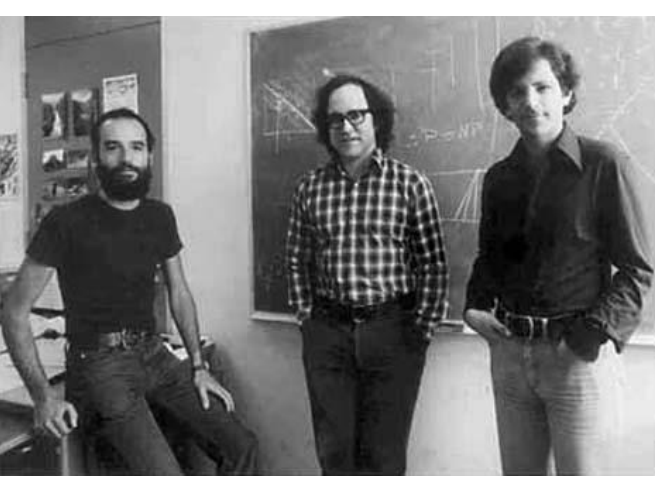
\includegraphics[width=72.66mm,height=132.46mm]{../../images/llm/page_003_img_01.png}%
\end{textblock*}

% deskripsi: Foto berwarna ketiga penulis RSA (Rivest, Shamir, Adleman) di masa tua mereka.
% bbox normalisasi: [0.5240, 0.3820, 0.9070, 0.8410]
\begin{textblock*}{80.43mm}(110.04mm,113.45mm)
\noindent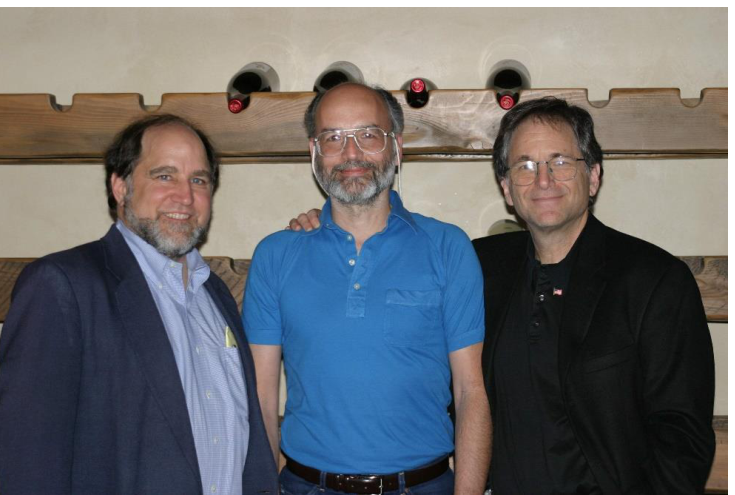
\includegraphics[width=80.43mm,height=136.32mm]{../../images/llm/page_003_img_02.png}%
\end{textblock*}

\end{document}
